\documentclass{article}
%\usepackage[a4paper, total={6in, 8in}]{geometry}
\usepackage{graphicx}
\graphicspath{ {C:\Users\harsh\OneDrive\Documents} }
\usepackage{geometry}
 \geometry{
 a4paper,
 total={210mm,297mm},
 left=20mm,
 right=20mm,
 top=-2mm,
 bottom=2mm,
 }

\usepackage{minted}
\newminted{python}{%
    % options to customize output of pythoncode
    % see section 5.3 Available options starting at page 16
}

\usepackage{hyperref}
 
%\usepackage[margin=0.5in]{geometry}
\usepackage{float}
\usepackage[caption = false]{subfig}
\usepackage[demo]{graphicx}
\usepackage{amsmath,amssymb}
\usepackage{ifpdf}
%\usepackage{cite}
\usepackage{algorithmic}
\usepackage{algorithm2e}
\usepackage{array}
\usepackage{mdwmath}
\usepackage{pdfpages}
\usepackage{mdwtab}
\usepackage{eqparbox}
\usepackage{algorithm}
% \usepackage{algpseudocode}
\usepackage{algpseudocode}
\usepackage{listings}
%\onecolumn
%\input{psfig}
\usepackage{color}
\usepackage{graphicx}
% \usepackage{hyperref}
\setlength{\textheight}{23.5cm} \setlength{\topmargin}{-1.05cm}
\setlength{\textwidth}{6.5in} \setlength{\oddsidemargin}{-0.5cm}
\renewcommand{\baselinestretch}{1}
\pagenumbering{arabic}
\renewcommand{\thesection}{\Roman{section}.} 
\renewcommand{\thesubsection}{\Alph{subsection}.}
\usepackage{xcolor}
\usepackage{titlesec}
% \titleformat{\section}[block]{\bfseries\large\filcenter}{}{5em}{}
\begin{document}

\textbf{
\begin{center}
{
\large{School of Engineering and Applied Science (SEAS), Ahmedabad University}\vspace{5mm}
}
\end{center}
%
\begin{center}
\large{\\
Probability and Stochastic Processes (MAT 277)\\ \vspace{4mm}
Special Assignment Report\\\vspace{4mm}
% Enrollment No: AUXXXXXXX \hspace{4cm} Name: XXXXX XXXXX
% Deadline : 24-02-2022 11:59 PM\\\vspace{2mm}
}
\end{center}}
\vspace{2mm}
\textbf{Group Name: hn\_tra\_27} \\

\textbf{Team Members:}
\begin{itemize}
    \item Utsav Raithatha (AU2140019)
    \item Ruchil Shah (AU2140119)
    \item Khushal Trivedi (AU2140125)
    \item Hardagna Mehta (AU2140144)
\end{itemize} \\

\textbf{Algorithm: Simulated Annealing}\\

\section{Team Activity Learning and Concept Map}
\begin{itemize}
    \large
    \item Team Activity Learnings:\\
    \begin{itemize}
        \item Collaborative problem solving was one of the main lessons the team learned from working on this special assignment. The team members needed to collaborate in order to comprehend the issue, collect data, and create a mathematical model in order to successfully resolve the vehicle routing challenge in ride-sharing systems.This required effective communication and collaboration among team members. \\
        \item To create a precise probabilistic model for the ride-sharing system, the team required to have a solid grasp of data analysis and mathematical modelling methods. This could entail creating mathematical models to replicate the behaviour of the system as well as utilising statistical techniques to analyse traffic patterns and user demand.Thus, data analysis and mathematical modelling were one of the key learnings.\\
        \item Team members learned proficient programming in  relevant language like Python in order to develop the Simulated Annealing technique and probabilistic modelling. This required not just building code to simulate the annealing process and generate routing solutions, but also comprehending the logic and execution of the algorithm.Thus, programming skills were also one of the learnings.\\

        \newpage
        \item To find the best method for resolving the vehicle routing problem, the team had to experiment with various Simulated Annealing algorithm settings and parameters by connecting ideas of probability to it. This would entail testing the algorithm's performance using various data sets and scenarios and fine-tuning it as required to get the best results.Thus experimentation and evaluation were also one of the team learnings.\\
    \end{itemize} \\

    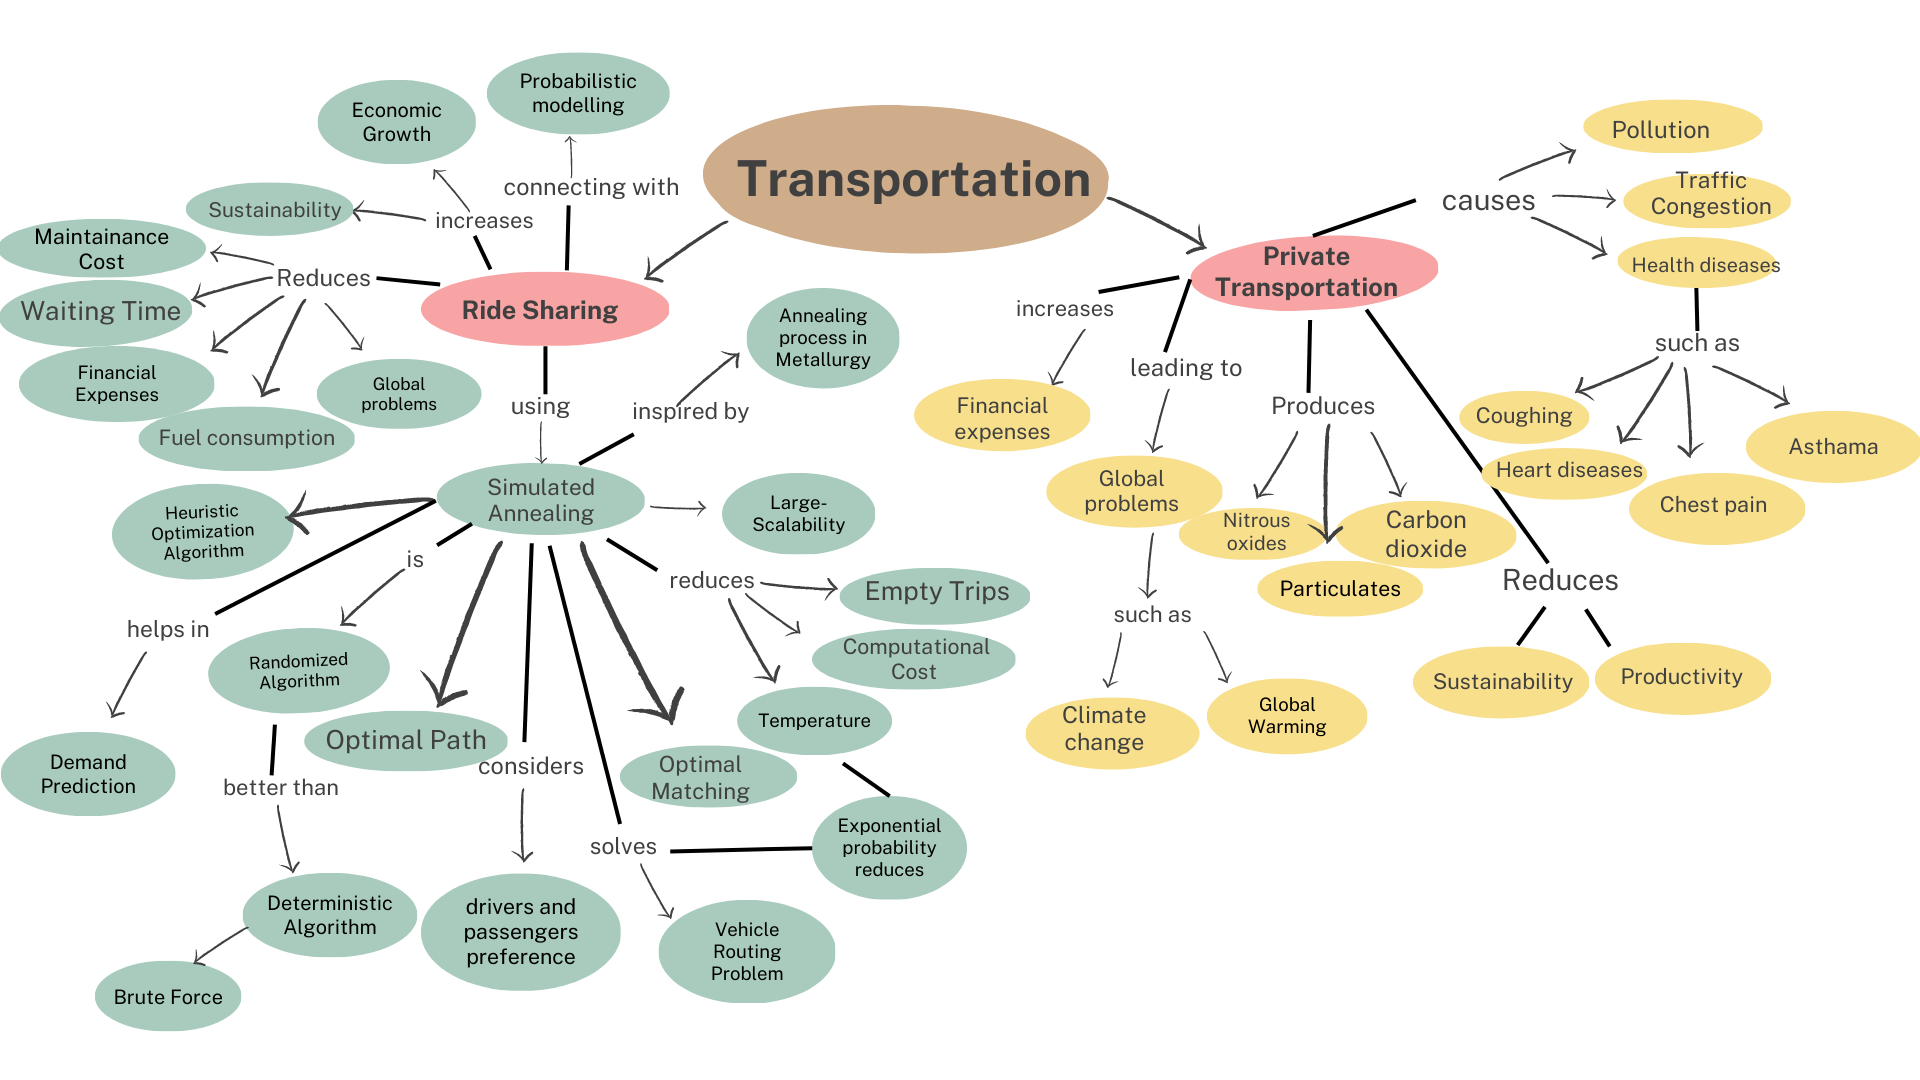
\includegraphics[scale = 0.34]{hn_tra_27_ConceptMap_27.png}
\end{itemize}
\newpage
\section{Background and Motivation}
\begin{itemize}
    \large
    \item The following is the background and motivation for addressing ride-sharing systems as a vehicle routing problem utilising probabilistic modelling and randomised algorithms:\\
    \item To begin with, ride-sharing systems are inherently dynamic and uncertain, with transportation demand shifting quickly and unpredictably. Traditional optimisation strategies may not be adequate in dealing with such uncertainty and unpredictability. Hence, probabilistic modeling can be used to capture this uncertainty and estimate the likelihood of various scenarios.\\
    \item Secondly, in ride-sharing systems, the vehicle routing problem is known to be computationally complex, especially when dealing with a high number of vehicles and passengers. Traditional optimisation techniques may necessitate a substantial amount of processing resources, making real-time vehicle routing optimisation difficult. Hence, randomized algorithms can be used to achieve faster computation times and more efficient routing solutions.\\
    \item Ride-sharing systems can optimise their routing decisions in real-time while accounting for the uncertainty and unpredictability inherent in these systems by using randomised algorithms in conjunction with probabilistic modelling. This method can lead to more efficient resource utilization, shorter journey times for consumers, and a better overall experience for everyone involved.\\
    \item The motivation behind choosing Simulated Annealing as randomized algorithm is that, solutions are found using a random search process, and the best solution is chosen using a set of random variables.The algorithm gradually reduces the level of randomness as it progresses, allowing it to converge on a more optimal solution over time. \\
    \item In summary, the background and motivation behind considering ride-sharing systems as a vehicle routing problem using probabilistic modeling and randomized algorithms is to address the complexity and uncertainty inherent in these systems while achieving faster computation times and more efficient routing solutions.\\
\end{itemize}
\newpage
\section{Algorithm Description}
\SetKwComment{Comment}{/* }{ */}

\begin{algorithm}
\caption{Simulated Annealing Algorithm}\label{alg:two}
\KwData{\text{current\_solution, temperature, cooling\_rate}}
\KwResult{\text{best\_solution}}
$\text{initial\_solution} \gets \text{generate initial random solution}$ \; \\
$\text{current\_solution} \gets \text{initial\_solution}$ \; \\
$\text{temperature} \gets 1000$\; \\
$\text{cooling\_rate} \gets 0.95$\; \\
\While{$\text{temperature} > 1$}{
    $\text{candidate\_solution} \gets \text{generate\_neighbour(current\_solution)}$\; \Comment*[r]{randomly find a neighbour}\\
    $\text{current\_objective} \gets \text{calculate\_objective(current\_solution)}$\; \Comment*[r]{objective function}\\
    $\text{candidate\_objective} \gets \text{calculate\_objective(candidate\_solution)}$\; \\ \\
  \eIf{$\text{candidate\_objective} < \text{current\_objective}$}{
    $ \text{current\_solution} \gets \text{candidate\_objective}$\; \\
    {\If{$\text{candidate\_objective} < \text{calculate\_objective(best\_solution)}$}{
      $\text{best\_solution} \gets \text{candidate\_objective}$\;
    }
  }
  }
  {$\text{acceptance\_probability} \gets exp(-(\text{candidate\_objective} - \text{current\_objective}) / temperature)$ \\
  \If{$random[0,1] < \text{acceptance\_probability}$}{
      $\text{current\_solution} \gets \text{candidate\_solution}$\; \Comment*[r]{accept the worse solution}
    }
  }   
  $\text{temperature} \gets \text{temperature}*\text{cooling\_rate}$ \Comment*[r]{update the temperature}
}
\end{algorithm}

\newpage

\begin{algorithm}
\caption{Ride Sharing Problem using Simulated Annealing Algorithm}\label{alg:two}
\KwData{Pickup and Drop-off locations of passengers and starting location of taxis}
\KwResult{Allocation of taxis to each passengers on shared basis and return the minimum cost i.e. distance travelled by all the taxis}

1. Generate an initial solution by randomly assigning passenger to each taxis according to capacity. \\

2. Generate a new solution by randomly swapping the passengers assigned to the taxi. \\

3. Evaluate the new solution using the objective function and calculate the total distance travelled. \\

4. Using the acceptance probability in simulated annealing, accept the solution or reject it based on the criterion of simulated annealing. \\

5. Repeat the simulated annealing process in step 2-4. \\

6. Output the passengers allocated to each taxi and return the best total distance travelled by all the taxis.

\end{algorithm}


\newpage
\begin{algorithm}
\caption{Ride Sharing Problem using Simple Brute Force}\label{alg:two}
\KwData{Pickup and Drop-off locations of passengers, starting location of taxis and taxi capacity}
\\
\KwResult{Allocation of taxis to each passengers on shared basis and return the minimum cost i.e. distance travelled by all the taxis}
\\ 1. Initialize the tour sequence to empty.
\\ 2. Generate all possible solutions (tours):
    \begin{itemize}
        \item Loop over all possible permutations of the passengers:
        \begin{itemize}
            \item For each permutation of passengers
            \item For each taxi location, add the combination of passengers that can be picked up and dropped off at that location to the tour sequence
        \end{itemize}
        \item Add the starting passenger location for each passenger to the tour sequence.
        \item Add the end passenger location for each passenger to the tour sequence.
    \end{itemize}
\\ 3. Calculate the total distance of the taxi trips in each tour sequence:
    \begin{itemize}
        \item For each taxi in the tour sequence:
        \begin{itemize}
            \item Calculate the distance traveled by the taxi from its initial location to the starting passenger location
            \item Add the distance traveled by the taxi from the starting passenger location to the end passenger location
            \item Add the additional distance traveled by the taxi from the end passenger location to its initial location
        \end{itemize}
    \end{itemize}
\\ 4. Choose the tour sequence with the lowest total distance:
    \begin{itemize}
        \item Save the selected tour sequence and the associated total distance
    \end{itemize}
\\ 5. Output the selected tour sequence and the associated total distance.
    

  
\end{algorithm}
 
\newpage
\section{Application} \\
\begin{itemize}
\large
    \item By splitting the cost of transportation, more space can be made available for other uses by lowering the number of automobiles parked in parking lots and on the streets. Ride-sharing services can ease urban traffic congestion by reducing the number of vehicles on the road.   \\

    \item By reducing the number of cars on the road and, consequently, their emissions, ride-sharing can help reduce carbon emissions. It can assist in lowering greenhouse gas emissions and air pollution. Thus, it helps in maintaining environmental sustainability. \\

    \item Ride-sharing can be a more affordable alternative to conventional modes of transportation like taxis or personal vehicles. People can split the expense of transportation by sharing rides, which can result in financial savings. Hence, this system is cost-effective.\\

    \item People who live in places lacking public transportation or have limited mobility may find ride-sharing more accessible. For those with impairments, ride-sharing firms frequently provide accessible vehicles and options, making it more straightforward for them to go around. Thus, this results in increased accessibility.  \\

    \item Companies that offer ride-sharing services often have safety procedures in place to guarantee the security of their customers. They carry out background checks on drivers, monitor rides in real time, and provide a system for rating both drivers and passengers. Hence, safety-related issues are also taken into consideration. \\

    \item Ride sharing services are often used for airport transportation, where passengers can share a ride to the airport and split the fare. This can be a cost-effective and convenient option for passengers who do not want to drive to the airport or park their cars at the airport. \\

    \item Ride sharing services are often used for special events such as concerts, sporting events, and festivals. Passengers can share a ride to the event and avoid the hassle of finding parking. \\

    \item Ride sharing services can be more efficient than traditional public transportation, as they are able to take passengers directly to their desired destinations. \\
    
    \item Ride sharing services are able to collect valuable data on traffic patterns, user behavior, and preferences, which can be used to optimize future transportation services. \\
\end{itemize}



\newpage
\section{Mathematical Analysis}
\large 

\textbf{Poisson Distribution Analysis of Car Pooling Problem:} \\

Let $X(t)$ be the number of taxis arriving at a particular location in time t. \\

Let i be the point of carpool position. The taxi car pool position meets the 

following conditions: \\

(1) $X(0) = 0$ which means that at $t = 0$ number of taxis is zero. \\

(2) $X(t)$ is an independent stationary increment process which means that the

probability of having a taxi within the time interval from $t$ to $t+h$ is

independent of $t$ and is proportional to the length of the interval h. \\

(3) $X(t)$ satisfies the following two formulas:
\begin{equation*}
    \begin{split}
        P\{X(t+h) - X(t) = 1\} = \lambda h + o(h) \\
        P\{X(t+h) - X(t) \geq 2\} = o(h)    
    \end{split}
\end{equation*}

where $o(h)$  is the function which is very less compared to h when h tends to 0.

The above equations means that the probability that the car pool position has only

one car is proportional to time interval h and more than or equal to two cars is 

negligible for small time interval h. \\

The probability that there are n taxis in the car pool position at time t is
\[P_n(t) = P\{X(t) = n\} = P\{X(t) - X(0) = n\}\]

Using the condition (2) and (3), we have, 
\begin{equation*}
    \begin{split}
        P_0(t+h) &= P\{X(t+h) = 0\} \\ 
        &= P\{X(t) - X(0) = 0\}P\{X(t+h) - X(t) = 0\} \\
        &= P_0(t)[1 - (\lambda h + o(h) + o(h))] \\
        &= P_0(t)[1 - \lambda h + 2o(h)] \\
    \end{split}
\end{equation*}

Let $ h \rightarrow 0$. So,

\begin{equation*}
    \begin{split}
        P_0(t+h) &= P_0(t)[1 - \lambda h] \\
        P_0(t+h) - P_0(t) &= - \lambda P_0(t) h \\
        \frac{P_0(t+h) - P_0(t)}{h} &= - \lambda P_0(t) \\
        \frac{d P_0(t)}{dt} &= - \lambda P_0(t) \\ 
        \frac{d P_0(t)}{P_0(t)} &= - \lambda dt \\
        ln P_0(t) &= - \lambda t \hspace{1cm} \text{(Integrating both sides)}\\
        P_0(t) &= e^{- \lambda t} 
    \end{split}
\end{equation*}
\newpage
Similarly we can have, $P_1(t) = \lambda t \, e^{- \lambda t}$ \\ 

And therefore, by mathematical induction we can have,
\[P_k = \frac{e^{- \lambda x}(\lambda x)^k}{k!}\] 

Therefore, the given situation follows a poisson process where $P_k$ indicates the

probability of reaching k cars within the counting interval x. $\lambda$ represents 

the average taxi arrival per unit time. \\

\textbf{Mathematical Analysis of Simulated Annealing Algorithm: } \\

The acceptance probability i.e. the probability to accept a worse solution while

finding an optimal solution in the simulated annealing is given by,

\[\text{Acceptance Probability} = exp \, \Big(- \frac{\Delta E}{T} \Big)\]

where $\Delta E = (\text{new state} - \text{current state})$ and \\ 

\hspace{1.2cm} $T = $ Previous Temperature * Cooling Rate \\

The cooling rate is less than one and close to one generally between 0.8 to 0.99 \\

So, the acceptance probability depends on $\Delta E$ and $T$. Acceptance probability will be

large if $\Delta E$ is less positive and Temperature is high. \\

Initially the temperature is high so the probability of accepting the worse solution initially

is high which should be the case as we don't want to stuck at local minima. Also if the 

new state is more worse then $\Delta E$ will be more positive making acceptance probability

lower.

\newpage

\section{Code(with description of each line)}
The following is the python code for solving the ride sharing problem using Simulated Annealing Algorithm.
\begin{pythoncode}
# Ride Sharing Problem using Simulated Annealing

import random
import math

# Calculating the distance for individual taxi
def total_distance(route):
  distance = 0
  for i in range(len(route)-1):
    distance += math.dist(route[i], route[i+1])
  return distance

# Objective function (total distance travelled by all the taxis) which is 
# to be minimized
def objective_function(solution):
  total_distance_travelled = 0
  for taxi in solution:
    taxi_location = taxi_locations[taxi]
    taxi_route = [taxi_location]
    passengers = solution[taxi]
    for passenger in passengers:
      passenger_start = passenger_locations[passenger]['start']
      passenger_end = passenger_locations[passenger]['end']
      taxi_route.append(passenger_start)
      taxi_route.append(passenger_end)
    taxi_route.append(taxi_location)
    total_distance_travelled += total_distance(taxi_route)
  return total_distance_travelled

# Randomly select an initial solution which will be optimized while
# doing simulated annealing
def generate_initial_solution():
  passengers = list(passenger_locations.keys())
  random.shuffle(passengers)
  solution = {}
  for i in range(0, len(passengers), taxi_capacity):
    taxi = 'taxi' + str(i // taxi_capacity + 1)
    solution[taxi] = passengers[i:i+taxi_capacity]
  return solution
\end{pythoncode}

\newpage

\begin{pythoncode}
# Implement simulated annealing
def simulated_annealing(initial_solution, temperature, cooling_rate):
  
  current_solution = initial_solution
  best_solution = current_solution
  
  while temperature > 1:
    new_solution = current_solution.copy()
    
    # Generate a new solution by swapping passengers between taxis
    taxi1 = random.choice(list(new_solution.keys()))
    taxi2 = random.choice(list(new_solution.keys()))
    while taxi1 == taxi2:
      taxi2 = random.choice(list(new_solution.keys()))
    passenger1 = random.choice(new_solution[taxi1])
    passenger2 = random.choice(new_solution[taxi2])
    new_solution[taxi1].remove(passenger1)
    new_solution[taxi2].remove(passenger2)
    new_solution[taxi1].append(passenger2)
    new_solution[taxi2].append(passenger1)

    # Calculate the cost of the new solution using objective function defined
    current_cost = objective_function(current_solution)
    new_cost = objective_function(new_solution)
    
    # Accept the new solution if it is better than the current solution
    if new_cost < current_cost:
      current_solution = new_solution
      
      # Compare the acceptance probability with a random number
      # generated between 0 and 1
      if objective_function(current_solution) < objective_function(best_solution):
        best_solution = current_solution
    
    # Accept the new solution based on acceptance probability and 
    # random number generated
    else:
      acceptance_probability = math.exp(-(new_cost - current_cost) / temperature)
      if random.random() < acceptance_probability:
        current_solution = new_solution
    
    # Reduce the temperature
    temperature *= cooling_rate

  return best_solution
\end{pythoncode}

\newpage

\begin{pythoncode}
# Pickup and Drop-off Locations of the passengers
passenger_locations = {
    'passenger1': {'start': (1,1), 'end': (3,3)},
    'passenger2': {'start': (2,2), 'end': (4,4)},
    'passenger3': {'start': (3,3), 'end': (5,5)},
    'passenger4': {'start': (4,4), 'end': (6,6)},
    'passenger5': {'start': (1,5), 'end': (8,3)},
    'passenger6': {'start': (2,6), 'end': (2,0)},
    'passenger7': {'start': (7,4), 'end': (4,2)},
    'passenger8': {'start': (2,3), 'end': (7,9)},
    'passenger9': {'start': (4,7), 'end': (5,2)},
    'passenger10': {'start': (7,9), 'end': (4,5)}
}

# Location of the taxis
taxi_locations = {
    'taxi1': (1,0),
    'taxi2': (7,8),
    'taxi3': (2,1),
    'taxi4': (3,2)
}

taxi_capacity = 3           # Capacity of passengers in each taxi

# Defining the parameters for simulated annealing
initial_solution = generate_initial_solution()
temperature = 1000
cooling_rate = 0.95

best_solution = simulated_annealing(initial_solution, temperature, cooling_rate)

print('Optimal allocation of passengers for each taxi: \n')
for taxi in best_solution:
  print(taxi + ': ' + str(best_solution[taxi]))
  
print('\nTotal distance travelled by all the taxis: ' +
                        str(objective_function(best_solution)))
\end{pythoncode}

\newpage

The following python code is for the deterministic approach to solve this problem.

However, it has a huge computational cost

\begin{pythoncode}
# Deterministic Approach to solve the Ride Sharing Problem

import math
from itertools import permutations

# Define the objective function
def total_distance(route):
  distance = 0
  for i in range(len(route)-1):
    distance += math.dist(route[i], route[i+1])
  return distance

# Objective function (total distance travelled by all the taxis) which is 
# to be minimized
def objective_function(solution):
  total_distance_travelled = 0
  for taxi in solution:
    taxi_location = taxi_locations[taxi]
    taxi_route = [taxi_location]
    passengers = solution[taxi]
    for passenger in passengers:
      passenger_start = passenger_locations[passenger]['start']
      passenger_end = passenger_locations[passenger]['end']
      taxi_route.append(passenger_start)
      taxi_route.append(passenger_end)
    taxi_route.append(taxi_location)
    total_distance_travelled += total_distance(taxi_route)
  return total_distance_travelled

# Find all the possible permutations of allocation of taxis to the passengers
def generate_all_possible_solutions():
  passengers = list(passenger_locations.keys())
  possible_solutions = []
  for perm in permutations(passengers):
    solution = {}
    for i in range(0, len(perm), taxi_capacity):
      taxi = 'taxi' + str(i // taxi_capacity + 1)
      solution[taxi] = perm[i:i+taxi_capacity]
    possible_solutions.append(solution)
  return possible_solutions

\end{pythoncode}

\newpage

\begin{pythoncode}    
# Find the minimum total distance travelled from all the possible solutions
def deterministic_algorithm():
  possible_solutions = generate_all_possible_solutions()
  best_solution = possible_solutions[0]
  best_cost = objective_function(best_solution)
  for solution in possible_solutions:
    cost = objective_function(solution)
    if cost < best_cost:
      best_solution = solution
      best_cost = cost
  return best_solution

# Pickup and Drop-off Locations of the passengers
passenger_locations = {
    'passenger1': {'start': (1,1), 'end': (3,3)},
    'passenger2': {'start': (2,2), 'end': (4,4)},
    'passenger3': {'start': (3,3), 'end': (5,5)},
    'passenger4': {'start': (4,4), 'end': (6,6)},
    'passenger5': {'start': (1,5), 'end': (8,3)},
    'passenger6': {'start': (2,6), 'end': (2,0)},
    'passenger7': {'start': (7,4), 'end': (4,2)},
    'passenger8': {'start': (2,3), 'end': (7,9)},
    'passenger9': {'start': (4,7), 'end': (5,2)},
    'passenger10': {'start': (7,9), 'end': (4,5)}
}

# Location of the taxis
taxi_locations = {
    'taxi1': (1,0),
    'taxi2': (7,8),
    'taxi3': (2,1),
    'taxi4': (3,2)
}

taxi_capacity = 3             # Capacity of passengers in each taxi


# Run the deterministic algorithm
best_solution = deterministic_algorithm()

# Print the best solution
print('Optimal allocation of passengers for each taxi:')
for taxi in best_solution:
  print(taxi + ': ' + str(best_solution[taxi]))

print('Total distance travelled by all the taxis: ' +
                            str(objective_function(best_solution)))
\end{pythoncode}

\newpage

\section{Results and Inferences}

The following is the plot for shared taxi allocated to almost 45 passengers and 20 taxis. We can see that as the iteration number increases i.e. the temperature decreases it approaches to the minimal total distance.

\begin{figure}[h]
\centering
{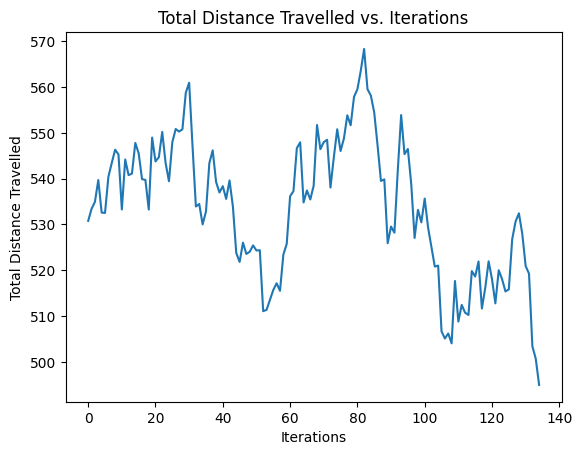
\includegraphics[width = 5in]{Total_Distance_Travelled_vs_Iterations.png}}  
\caption{Total Distance Travelled vs Iterations}
\label{some example}
\end{figure}

The time complexity of the Randomized approach is $O(n^2)$ because it largely depends on the distance calculation function which takes $O(n^2)$. \\

However, the time complexity of the deterministic approach which gives the perfect answer is very large i.e. $O(n!)$ as it finds all the permutations to calculate the minimum answer. \\

So, the randomized approach makes sense in the real life scenario.

\newpage
\section{References}
\\
\url{https://machinelearningmastery.com/simulated-annealing-from-scratch-in-python/#:~:text=Simulated%20Annealing%20is%20a%20stochastic,algorithms%20do%20not%20operate%20well.} \\

\url{https://www.researchgate.net/publication/327539965_Method_of_Taxi_Carpooling_Probability_and_Wait_Time_Based_on_Poisson_Distribution} \\

\url{https://github.com/jedrazb/python-tsp-simulated-annealing/blob/master/simulated_annealing.py} \\

\url{https://www.researchgate.net/publication/281445468_Dynamic_Shared-Taxi_Dispatch_Algorithm_with_Hybrid_Simulated_Annealing}

\end{document}